\documentclass[11pt,a4paper]{article}
\usepackage[T1]{fontenc}
\usepackage[margin=1in]{geometry}
\usepackage{amsmath,amssymb,mathtools,amsthm}
\usepackage{booktabs}
\usepackage{graphicx}
\usepackage{xcolor}
\usepackage[colorlinks=true,linkcolor=blue!60!black,citecolor=blue!60!black,urlcolor=blue!60!black]{hyperref}
\usepackage{microtype}
\usepackage{xurl}
\setlength{\emergencystretch}{3em}
\usepackage{enumitem}
\usepackage[most]{tcolorbox}
\usepackage{longtable}
\usepackage{float}
\newtcolorbox{keybox}[1][]{colback=blue!3,colframe=blue!45!black,boxrule=0.5pt,left=4pt,right=4pt,top=3pt,bottom=3pt,#1}
\newtcolorbox{failbox}[1][]{colback=red!3,colframe=red!45!black,boxrule=0.5pt,left=4pt,right=4pt,top=3pt,bottom=3pt,#1}
\newtheorem{theorem}{Theorem}
\newtheorem{lemma}{Lemma}
\newcommand{\elat}{e_{\mathrm{lat}}}
% generated by exploration/exciton/python/phase1_paper_numbers.py -- do not edit
\newcommand{\SzeroAdamsRhs}{400}
\newcommand{\SzeroAdamsErr}{$9.76\times10^{-10}$}
\newcommand{\SzeroBdfErr}{$3.11\times10^{-7}$}
\newcommand{\KAaRel}{$1.35\times10^{-8}$}
\newcommand{\KAbRel}{$1.08\times10^{-15}$}
\newcommand{\KAcRel}{$7.23\times10^{-15}$}
\newcommand{\KAtwoRel}{$8.06\times10^{-13}$}
\newcommand{\KAfourRel}{$8.75\times10^{-14}$}
\newcommand{\KAthreeHess}{$4.97\times10^{-9}$}
\newcommand{\KAcAtwoRel}{$2.25\times10^{-13}$}
\newcommand{\KAthreeE}{$5.23\times10^{-14}$}
\newcommand{\KAthreeF}{$6.39\times10^{-16}$}
\newcommand{\FFworstRel}{$1.68\times10^{-12}$}
\newcommand{\FFBcmT}{55.9}
\newcommand{\FFBcRel}{$1.57\times10^{-12}$}
\newcommand{\FFspinNum}{0.730}
\newcommand{\FFspinCF}{0.7254}
\newcommand{\FFstarts}{600}
\newcommand{\SandA}{44.7}
\newcommand{\SandB}{14.2}
\newcommand{\SandC}{4.64}
\newcommand{\SandD}{2.87}
\newcommand{\SandE}{1.87}
\newcommand{\SandF}{1.44}
\newcommand{\SandNA}{22.4}
\newcommand{\SandNB}{13.0}
\newcommand{\SandNC}{10.1}
\newcommand{\SandND}{8.26}
\newcommand{\PtwoAdev}{$1.85\times10^{-14}$}
\newcommand{\PtwoAom}{$1.57\times10^{-15}$}
\newcommand{\PtwoBom}{$5.77\times10^{-11}$}
\newcommand{\PtwoBomTwo}{$1.15\times10^{-10}$}
\newcommand{\PtwoBre}{$2.39\times10^{-11}$}
\newcommand{\PtwoCom}{$6.33\times10^{-9}$}
\newcommand{\PtwoCn}{16}
\newcommand{\LEANNEW}{Lean 4.34.1 with Mathlib tag v4.34.1 (commit d13f23b7)}
\newcommand{\NRuns}{2860}
\newcommand{\NRunsCM}{2060}
\newcommand{\NRunsN}{800}
\newcommand{\NCases}{21}
\newcommand{\NNotConv}{1404}
\newcommand{\NLtwoViol}{0}
\newcommand{\NCommTotal}{9}
\newcommand{\NCommAttained}{8}
\newcommand{\NMinRatio}{$-1.1\times10^{-13}$}
\newcommand{\NFrusMin}{$7.9\times10^{-7}$}
\newcommand{\NFrusMax}{$8.6\times10^{-3}$}
\newcommand{\NNoneBest}{0.663}
\newcommand{\NNoneWorst}{0.724}
\providecommand{\NPARTABSTRACT}{}
\providecommand{\VERIFYSTATUS}{}

\newcommand{\DaWorstN}{$1.2\times10^{-12}$}
\newcommand{\DaWorstNR}{$5.9\times10^{-14}$}
\newcommand{\DaWorstOm}{$4.8\times10^{-13}$}
\newcommand{\DaBelowPsi}{$1.6\times10^{-11}$}
\newcommand{\DbMatch}{$2.7\times10^{-9}$}
\newcommand{\DbMaxRe}{$1.4\times10^{-10}$}
\newcommand{\DcNorm}{$1.6\times10^{-11}$}
\newcommand{\DcEnergy}{$4.1\times10^{-10}$}
\newcommand{\DcSteps}{6464}
\newcommand{\DdBudgetMax}{$5.0\times10^{-7}$}
\newcommand{\DdResidMax}{$3.9\times10^{-4}$}
\newcommand{\DdResidZero}{$1.6\times10^{-7}$}
\newcommand{\DdBudgetZero}{$2.5\times10^{-15}$}
\newcommand{\DdShiftA}{0.0488}
\newcommand{\DdCentreA}{7.07}
\newcommand{\DdCornerA}{11.08}
\newcommand{\DdJA}{$7.6\times10^{-3}$}
\newcommand{\DdShiftB}{0.0876}
\newcommand{\DdCentreB}{4.58}
\newcommand{\DdCornerB}{11.92}
\newcommand{\DdJB}{$1.3\times10^{-2}$}
\newcommand{\DdShiftC}{0.1422}
\newcommand{\DdCentreC}{1.49}
\newcommand{\DdCornerC}{13.06}
\newcommand{\DdJC}{$1.2\times10^{-2}$}
\newcommand{\DdOmegaZero}{0.500000}
\newcommand{\DdMaxReLambda}{$9.2\times10^{-6}$}
\newcommand{\ExplResid}{$1.0\times10^{-8}$}
\newcommand{\ExplBudget}{$1.1\times10^{-13}$}
\newcommand{\ExplOmega}{0.587610}
\newcommand{\ExplOtherSentence}{the other amplitudes give $V_0=0$: residual $3.3\times10^{-10}$, budget $0.0\times10^{0}$; $V_0=0.25$: residual $6.0\times10^{-8}$, budget $2.4\times10^{-14}$; $V_0=1$: residual $8.7\times10^{-9}$, budget $6.9\times10^{-13}$ (all within the registered thresholds).}
\newcommand{\ExplRtolResid}{$7.6\times10^{-5}$}
\newcommand{\DeTraj}{$7.3\times10^{-6}$}
\newcommand{\DfRatioA}{4.20}
\newcommand{\DfRatioB}{4.07}
\newcommand{\DgN}{220.0}
\newcommand{\DgBudget}{0.52}
\newcommand{\DgSeeds}{3}
\newcommand{\NPARTABSTRACTTHREE}{the steady states, the $768\times768$ linearisation (matched to $2.7\times10^{-9}$), the conservative limit and the IMEX threshold and order passed as registered; the stationarity and pump-budget gates of the gate sweep \emph{failed} as registered at $t=4000$ (residual up to $3.9\times10^{-4}$; the horizon was too short for the slow relaxation) and pass in an exploratory continuation to $t=16000$, one seed per amplitude; the hypothesis that the emission shift lies between $0$ and $V_0$ held at all three gate amplitudes.}


\title{\textbf{Gated exciton fluids:}\\
a proof that image charges preserve complete monotonicity, a driven-dissipative solver test on rusty-SUNDIALS,\\
and a laboratory protocol}
\author{Xavier Callens\\ \small SocrateAI Research\\
\small \url{https://github.com/xaviercallens/SocrateAI-Scientific-QuantumFluids}}
\date{October 2026}
\hypersetup{pdftitle={Gated exciton fluids},pdfauthor={Xavier Callens},pdfsubject={Image-charge kernels, driven-dissipative GPE, laboratory protocol}}

\begin{document}
\begin{center}
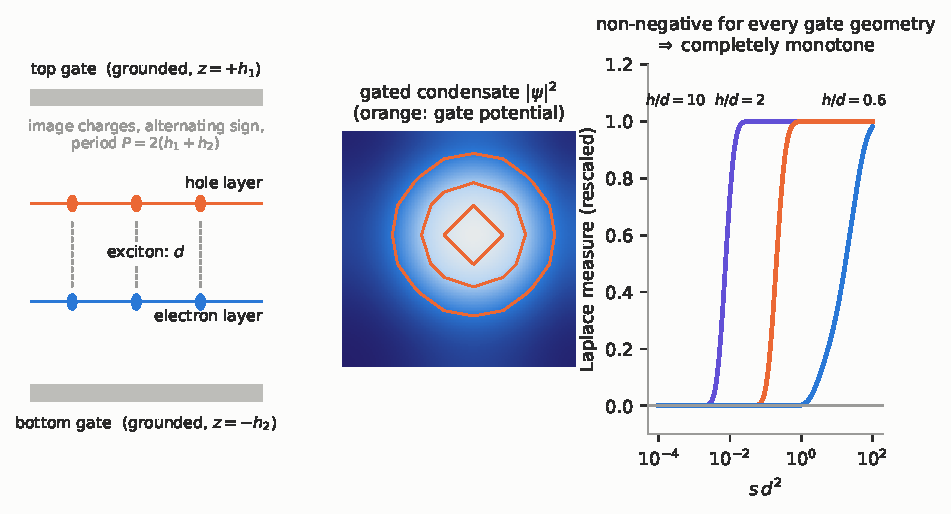
\includegraphics[width=0.97\textwidth]{figs_exciton3/fig_cover.pdf}
\end{center}
\vspace{-0.8em}
\begin{center}
{\Large\textbf{Gated exciton fluids:}\\[2pt]
\large a proof that image charges preserve complete monotonicity, a driven-dissipative solver test\\ on rusty-SUNDIALS, and a laboratory protocol}\\[8pt]
Xavier Callens\\ {\small SocrateAI Research \quad\url{https://github.com/xaviercallens/SocrateAI-Scientific-QuantumFluids}}\\[2pt]
{\small October 2026}
\end{center}
\vspace{-0.4em}

\begin{abstract}\small\noindent
A planar universal-optimality theorem for completely monotone interactions (OpenAI, September 2026~\cite{OpenAI2026}; AI-generated, unrefereed) was
used in a first note~\cite{CallensExciton1} as a dependency check on the exciton--exciton interaction of a 2026 bilayer experiment.
That note left open whether the \emph{dual-gated} device kernel, a sum of image charges of alternating sign, is completely monotone
in $r^2$ (numerical evidence only), and whether gates could be engineered to break it. Here we \textbf{prove} (Theorem~1, paper
and pencil, not in Lean) that for ideal grounded metal gates at arbitrary distances and arbitrary layer positions, the
Laplace measure of the kernel in $r^2$ is a sum of manifestly non-negative terms,
$S_m=2\bigl(1-\cos(b-a)\bigr)\bigl(1+\cos(a+b)\bigr)$; the gates therefore cannot break complete monotonicity in this model. A
by-product is the zero-wavevector coefficient $\tilde U(0)=4\pi d\,(1-d/D)$ for a gate separation $D$ (a capacitor formula,
not new; the mean-field baseline of the protocol). A spectral argument supplied by an independent reviewer extends the theorem to any
laterally homogeneous layered dielectric between grounded planes (Section~\ref{sec:cm}). Second, we test the solver stack on the model the experiment's community
would use for short-lived excitons or polaritons, a driven-dissipative Gross--Pitaevskii equation with an incoherent reservoir
and a gate potential, in a pre-registered design with known answers: \NPARTABSTRACTTHREE{} We report what failed or had to be
changed (a registered cost was misjudged by two orders of magnitude; three amendments were written before the numbers they affect, a
fourth while the last run was in progress, and one registered comparison was replaced by a better-posed one). Third, we give a laboratory protocol, and say which of its items can fail and which are controls. We do not use
Hugging Face materials data or neural-network surrogates, do not compare with data, and make no claim about exciton
Bose--Einstein condensation. Written by an AI system; not refereed.
\end{abstract}

\section{Why this note, and what it is not}

The request that prompted this note asked for a driven-dissipative exciton fluid on rusty-SUNDIALS with materials data from Hugging Face.
The first note~\cite{CallensExciton1} did something else (conservative gradient flows, a lattice theorem). We say so
because the two are easily confused: that note did \emph{not} contain a driven-dissipative model, an ARKode-type integrator, a
gate, a defect, or any materials input. This one adds the first three in a minimal form (Section~\ref{sec:dd}) and tests the
ARKode-style module that exists in the library; it does not add the last (Section~\ref{sec:notdone}).

\begin{keybox}
\textbf{What is established here.} (i) Theorem~1 below, a short exact argument (checked numerically on 300 random geometries).
(ii) Registered numerical gates on a standard open-dissipative model: which passed, which failed, in
Section~\ref{sec:results}. \textbf{What is not.} No quantum phase transition is located; no experiment is
reproduced; the model parameters are dimensionless and not those of any device; the protocol of Section~\ref{sec:protocol} is a
proposal that nobody has run.
\end{keybox}

\section{Gated kernels are completely monotone}\label{sec:cm}

\paragraph{Setting.} Grounded perfect-conductor planes at $z=+h_1$ and $z=-h_2$; a homogeneous dielectric between them (a uniform
$\varepsilon$ is a prefactor, an anisotropic one rescales $z$ by a constant); an electron layer at $z_e$ and a hole layer at
$z_h=z_e+d$. The exciton--exciton kernel is $U=V_{ee}+V_{hh}-2V_{eh}$, $V$ the Green function of the box. With
$P=2(h_1+h_2)$ a unit charge at $z_0$ produces at $(z,r)$
\[
V(z,z_0;r)=\sum_{n\in\mathbb Z}\Bigl[\bigl(r^2+(z-z_0-Pn)^2\bigr)^{-1/2}-\bigl(r^2+(z-2h_1+z_0-Pn)^2\bigr)^{-1/2}\Bigr].
\]

\begin{theorem}\label{thm:cm}
$U$ is completely monotone as a function of $t=r^2$ on $(0,\infty)$: $U=\int_0^\infty e^{-st}\mu(s)\,ds$ with $\mu\geq0$.
\end{theorem}

\begin{proof}
Write each term as $(t+a^2)^{-1/2}=\pi^{-1/2}\int_0^\infty e^{-s(t+a^2)}s^{-1/2}ds$. Then $\mu(s)=(\pi s)^{-1/2}S(s)$ where $S(s)$ is
the sum over images of $e^{-sa^2}$ with the signs of $V_{ee}+V_{hh}-2V_{eh}$. Poisson summation,
$\sum_n e^{-s(c+Pn)^2}=(\pi/s)^{1/2}P^{-1}\sum_{m\in\mathbb Z}e^{-\pi^2m^2/(P^2s)}\cos(2\pi mc/P)$, gives
$S(s)=(\pi/s)^{1/2}P^{-1}\sum_m e^{-\pi^2m^2/(P^2s)}S_m$ with, for $\alpha=2\pi m/P$, $a=\alpha(z_e-h_1)$, $b=\alpha(z_h-h_1)$
(so $\alpha d=b-a$),
\[
S_m=2-\cos2a-\cos2b-2\cos(b-a)+2\cos(a+b)=2\bigl(1-\cos(b-a)\bigr)\bigl(1+\cos(a+b)\bigr)\geq0,
\]
using $\cos2a+\cos2b=2\cos(a+b)\cos(a-b)$; and $S_0=0$ by neutrality. Hence $S(s)\ge0$ termwise.
\end{proof}

\begin{figure}[ht]
\centering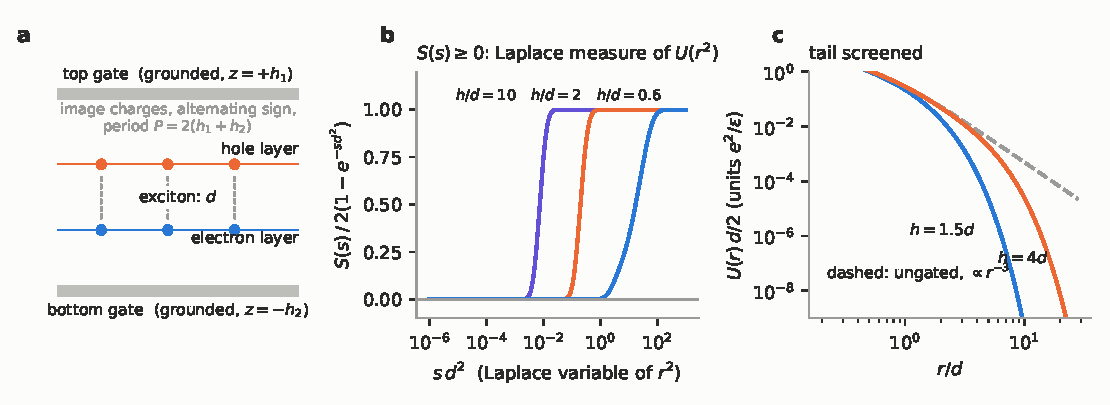
\includegraphics[width=\textwidth]{figs_exciton3/fig_cm_gates.pdf}
\caption{(a) The device and its image series. (b) $S(s)/2(1-e^{-sd^2})$ from the exact Poisson form for three symmetric gate
distances: non-negative everywhere, as Theorem~1 states. (c) The kernel with and without gates: the gates remove the dipolar
$r^{-3}$ tail (exponential screening at $r\gg h$) without leaving the completely monotone class. All three panels are generated
from the formulas of the text by \texttt{phase3\_figures.py}.}
\end{figure}

\paragraph{Consequences, and limits of the claim.} The single-gate and gate-free limits are pointwise limits of completely
monotone functions and so are completely monotone. Within \emph{this} model the gates cannot be engineered to violate the
hypothesis of the lattice theorem; if Kagome or stripe ground states are observed in a gated device, then, \emph{conditionally on the
unrefereed lattice theorem}, they come from something the model leaves out: lateral inhomogeneity, finite screening of real gates,
disorder, or quantum fluctuations.

\paragraph{Remark (layered dielectrics; due to the independent review of this note, not proved here in detail).} For a laterally
homogeneous layered dielectric $\varepsilon(z)$ between the grounded planes, expanding the Green function in the Dirichlet
Sturm--Liouville modes $-(\varepsilon\phi')'=\lambda\varepsilon\phi$ gives
$U(r)=2\sum_m\bigl(\phi_m(z_e)-\phi_m(z_h)\bigr)^2K_0(\sqrt{\lambda_m}\,r)$, a positive combination of $K_0(\kappa r)=\tfrac12\int_0^\infty
e^{-u-\kappa^2r^2/4u}\,du/u$, each completely monotone in $r^2$. So dielectric image charges of weight $\kappa^n$ do not break the property
either; the reviewer checked the expansion numerically on one four-layer stack. We have not repeated that check and have not written the full argument.
The same sum-of-squares structure is behind $S_m=2(\sin a-\sin b)^2$. The lattice theorem itself is imported and was not refereed.
A Lean formalisation needs the Poisson summation of Mathlib's Jacobi theta; we did not do it. The zero-wavevector coefficient
follows from the same series (and from Gauss's law for three capacitors in series), for a uniform $\varepsilon$ in units $e^2/\varepsilon=1$:
\begin{equation}\label{eq:u0}
\tilde U(0)=\int U\,d^2r=4\pi d\,\Bigl(1-\frac dD\Bigr),\qquad D=h_1+h_2 .
\end{equation}
We checked it against the numerical integral of the image series (agreement to $3\times10^{-3}$ relative at $D=3d$ and $D=20d$, limited by the integration cutoff).
It is a capacitor formula, textbook. For piecewise $\varepsilon$ the factor $1-d/D$ becomes $1-(d/\varepsilon_m)/\sum_it_i/\varepsilon_i$ (Gauss's law with layers $t_i$ of permittivity $\varepsilon_i$ between the gates, $\varepsilon_m$ between the exciton layers), which changes the size of the $D$-dependence for hBN-encapsulated stacks. It is the \emph{mean-field} coefficient: valid at densities where correlations are weak (Section~\ref{sec:protocol}, L1).

\section{A driven-dissipative model with a gate, tested on rusty-SUNDIALS}\label{sec:dd}

\paragraph{Model.} Dimensionless units $\hbar=m=1$,
\begin{align}
i\,\partial_t\psi &= \Bigl[-\tfrac12\nabla^2+V(\mathbf x)+g|\psi|^2+g_Rn_R+\tfrac i2\bigl(Rn_R-\gamma\bigr)\Bigr]\psi,\\
\partial_tn_R&=P(\mathbf x)-(\gamma_R+R|\psi|^2)n_R,
\end{align}
the standard open-dissipative (Wouters--Carusotto~\cite{WoutersCarusotto2007}) form with $g=0.04$, $g_R=1$, $\gamma=0.1$, $\gamma_R=200$, $R=1$ (stiff ratio
$\gamma_R/\gamma=2000$), uniform pump $P$ and gate $V=V_0e^{-d^2/2\sigma^2}$. Above threshold $P_{th}=\gamma\gamma_R/R=20$ the
uniform state is $n=P/\gamma-\gamma_R/R$, $n_R=\gamma/R$, $\omega=gn+g_Rn_R+V$ (we use $P=21$: $n=10$, $n_R=0.1$, $\omega=0.5$).
The model is generic; it is the form one would write for short-lived excitons or polaritons, but with reservoir parameters chosen for solver stiffness (a reservoir $2000$ times faster than the condensate, $g_R/g=25$), not measured ones; real reservoirs are typically slower than the condensate. It is \emph{not} the model of the
equilibrium experiment of Qi \emph{et al.}~\cite{Qi2026}, whose dipolar excitons live microseconds.

\paragraph{Design.} Pre-registered in \path{docs/designs/EXCITON_FLUID_PHASE3_PREREG.md} (commit \texttt{335caa5}, before any run of the
Rust program), independent Python reference first (\path{phase3_reference.py}). Gates: D-a steady states above and below threshold;
D-b the 768$\times$768 linearisation of the solver against the reference $3\times3$ per-$k$ spectrum; D-c conservative limit
(norm and energy); D-d gate sweep ($V_0\in\{0,0.25,0.5,1\}$): pump budget $\sum P=\sum(\gamma_Rn_R+\gamma|\psi|^2)$, single locked
frequency, and the hypothesis $0<\omega(V_0)-\omega(0)<V_0$; D-e the ARKode-style IMEX module, whose implicit stage is a fixed-point
iteration and so must fail when $h\gamma_Ra_{ii}\geq1$ (bracketed by five step sizes only); D-f its temporal order; D-g a planted bug. A deliberately
\emph{wrong} prediction is excluded by construction: the intuitive local-density guess that the gate leaves the density pinned at
$P/\gamma-\gamma_R/R$ is incompatible with a single locked frequency (the gate shifts the local frequency, so currents must flow),
and was not registered.

\paragraph{Amendments and disclosures.} A1--A3 were written before the numbers they affect; A4 (D-g was evaluated on three
of ten seeds, from the per-seed log lines, because the planted-bug runs take about 25 minutes each) was recorded while D-g was
running and committed with the results. A1: the IMEX module's fixed-point test squares the tolerance
(effective absolute tolerance $\mathrm{rtol}\,(\mathrm{atol}+\mathrm{rtol}|z|)$), so $10^{-12}$ cannot converge in floating point;
set to $10^{-6}$. A2: integrating D-a/D-d/D-g in the laboratory frame needed more than 23 minutes for one run (the phase rotates
at $\omega=0.5$ and BDF must resolve it for $t=4000$); the flow is integrated in the frame rotating at the registered value of
$\omega$ with all gate quantities evaluated gauge-covariantly. A3: even then the pinned CVODE refactors a dense matrix
every few steps (43 ms per step at 768 unknowns, hours per run, about 70 runs), so \textbf{D-a, D-d, D-g were run on an
$8\times8$ grid with $\sigma=1.5$} (same $\sigma/L$), not $16\times16$; D-b, D-c, D-e, D-f ran on $16\times16$ as registered.
\emph{The $8\times8$, $\sigma=1.5$ problem is not equivalent to the registered $16\times16$, $\sigma=3$ one} (Section~\ref{sec:results}):
the consequence is that the gate-sweep results describe a very small box. Further disclosures: (i) D-b was registered as a comparison of the two
\emph{sorted} eigenvalue lists; as implemented it gives a maximum difference $18.2$ because sorting by (real, imaginary) is unstable
for nearly degenerate pairs, and the reported $2.7\times10^{-9}$ is from a nearest-neighbour matching introduced in the summariser
without an amendment, which should have been one; the Jacobian itself was reconstructed independently by the reviewer and agrees.
(ii) Exploratory runs launched to test the horizon were first made with a stale binary that ignored the overrides (results identical to
$t=4000$); they are kept under \path{results/phase3/exploratory_invalid/} and were not used. (iii) The first, laboratory-frame attempt
and the stopped $16\times16$ rotating-frame attempt are kept as logs under \path{results/phase3/}.

\section{Results of the registered gates}\label{sec:results}

\begin{table}[ht]
\centering\small
\begin{tabular}{@{}p{0.09\textwidth}p{0.075\textwidth}p{0.5\textwidth}p{0.2\textwidth}@{}}
\toprule
gate & grid & outcome (numbers from \texttt{summary.json}) & registered result \\ \midrule
D-a & $8\times8$ & above threshold, 10 seeds started at the closed form plus $10^{-3}$ noise (a stability check, not a basin test): relative $n$, $n_R$ and absolute $\omega$ deviations \DaWorstN{}, \DaWorstNR{}, \DaWorstOm{}; below: $\max|\psi|\le$ \DaBelowPsi{} & pass \\
D-b & $16\times16$ & eigenvalues of the solver's $768\times768$ finite-difference Jacobian matched one-to-one to the reference to \DbMatch{}; largest real part \DbMaxRe{} (the Goldstone mode). \emph{The registered sorted comparison gives $18.2$; see Section~\ref{sec:dd}} & pass with a replaced criterion \\
D-c & $16\times16$ & norm drift \DcNorm{}, energy drift \DcEnergy{} over $t=20$ (\DcSteps{} steps) & pass \\
D-d (i),(ii) & $8\times8$ & pump budget up to \DdBudgetMax{} (gate $10^{-8}$), stationarity residual up to \DdResidMax{} (gate $10^{-7}$); even $V_0=0$ gives \DdResidZero{} & \textbf{fail} \\
D-d (iii) & $8\times8$ & $\omega(V_0)-\omega(0)=$ \DdShiftA{}, \DdShiftB{}, \DdShiftC{} for $V_0=0.25,0.5,1$: between $0$ and $V_0$, increasing (medians at $t=4000$); in this box this is the area average of the gate, see text & pass (hypothesis; uninformative) \\
D-e & $16\times16$ & one step succeeds at $h=0.005,0.01,0.0125$ and returns an error at $0.02,0.05$ (threshold $0.01707$); no silent non-finite result; trajectory to $t=20$ within \DeTraj{} of CVODE & pass \\
D-f & $16\times16$ & error ratios \DfRatioA{} and \DfRatioB{} on halving $h$ (second order) & pass \\
D-g & $8\times8$ & planted bug: $n=$ \DgN{} instead of $10$; budget violated by $\ge$\DgBudget{} (\DgSeeds{} seeds, amendment A4) & pass \\
\bottomrule
\end{tabular}
\caption{Gates as registered. Every number is generated from the run records by \texttt{phase3\_paper\_numbers.py}.}
\end{table}

\begin{figure}[ht]
\centering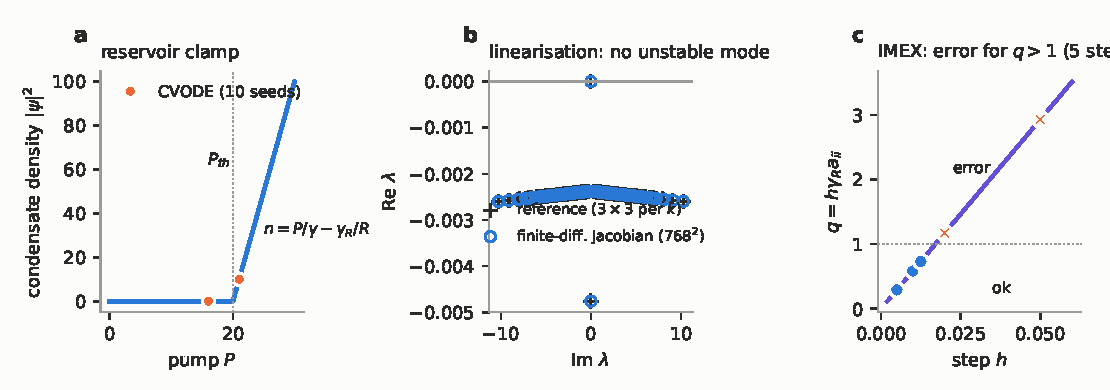
\includegraphics[width=\textwidth]{figs_exciton3/fig_solver.pdf}
\caption{Solver tests. (a) Steady-state density against pump: closed form (line) and ten CVODE runs per pump (dots; they
coincide to \DaWorstN{}). (b) The eigenvalues of a central-difference Jacobian of the solver's right-hand side (circles) lie on the reference spectrum
(crosses); the isolated points are the $k=0$ phase (Goldstone) and amplitude modes; the fast reservoir mode near $-\gamma_R$ is outside the plotted range. (c) The IMEX module's fixed-point stage:
contraction factor $q=h\gamma_Ra_{ii}$; it returns an error for $q=1.17$ and $2.93$ and succeeds for $q\leq0.73$ (the threshold $q=1$ is bracketed, not located).}
\end{figure}

\begin{failbox}
\textbf{The registered gate-sweep gates failed.} At $t=4000$ the stationarity residual of the gated states is up to \DdResidMax{}
and the pump budget is violated by up to \DdBudgetMax{}, against thresholds $10^{-7}$ and $10^{-8}$; the ungated state also
exceeds its threshold (\DdResidZero{}). The horizon was set from the decay rate of the ungated Bogoliubov modes ($2.4\times10^{-3}$) applied to a $10^{-3}$ perturbation;
the gated states start $O(0.1)$ from the uniform state and the slowest linear decay rates about them are $1.4$--$2.1\times10^{-3}$
(reviewer's linearisation), so $e^{-1.4\times10^{-3}\cdot4000}\approx3\times10^{-3}$ of an $O(0.1)$ amplitude is left. The ungated failure
($1.6\times10^{-7}$) was predictable from the registered numbers. All ten seeds end on the same state to all printed digits, and the
residual does not depend on the integrator tolerance ($\mathrm{rtol}=10^{-8}$ to $10^{-12}$ give \ExplRtolResid{}), so it is not
integration error. \emph{Exploratory} continuations (not gates, one seed each) to $t=16000$ give residual \ExplResid{} and budget
violation \ExplBudget{} for $V_0=0.5$, which would pass; \ExplOtherSentence{}
\end{failbox}

\begin{figure}[ht]
\centering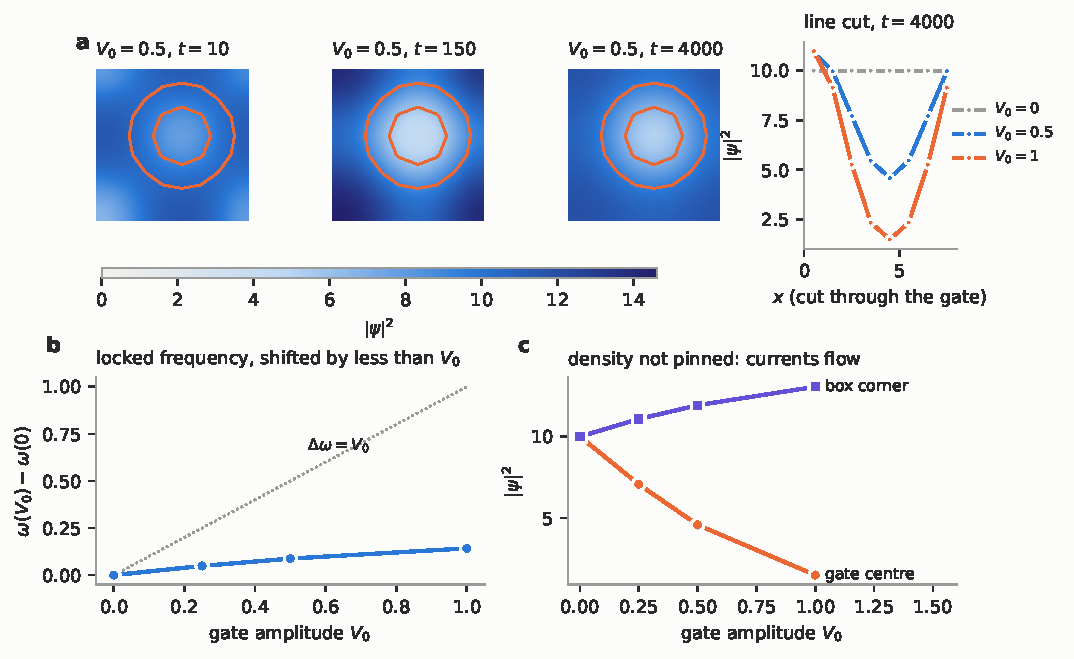
\includegraphics[width=\textwidth]{figs_exciton3/fig_gate.pdf}
\caption{A gated driven-dissipative condensate on the $8\times8$ grid ($\sigma=1.5$), uniform pump $P=21$.
(a) Density from the uniform start with noise at three times (orange: contours of the gate; fields are
bicubic interpolations of the $8\times8$ values) and a line cut through the gate at $t=4000$ for three amplitudes.
(b) The locked emission frequency shifts with the gate amplitude by less than $V_0$; in this small box that is the area average of the gate (text).
(c) Density at the gate centre falls and at the box corner rises: the density is \emph{not} pinned at its ungated value,
because the single locked frequency requires currents (largest current density
\DdJA{}--\DdJB{} for $V_0=0.25$--$0.5$).}
\end{figure}

\paragraph{What the gate sweep shows, and does not show.} In the small box the gate depletes the condensate at its centre
(from $10$ to \DdCentreA{}, \DdCentreB{}, \DdCentreC{} for $V_0=0.25,0.5,1$, while the corner rises to \DdCornerA{}, \DdCornerB{},
\DdCornerC{}), and currents flow. The single emission frequency moves by \DdShiftA{}, \DdShiftB{}, \DdShiftC{}.
\emph{That shift is a box-size artefact and carries little information.} An independent re-solution of the same stationary states by the
reviewer (own Newton solver; it reproduces the shifts to five digits) at fixed gate width $\sigma=1.5$ gives, for $V_0=1$,
$0.142$ ($L=8$), $0.024$ ($L=16$), $0.0055$ ($L=32$): $\Delta\omega$ falls like $L^{-2}$ and at small $V_0$ equals the area average
of the gate, $V_0\,2\pi\sigma^2/L^2$. ``Between $0$ and $V_0$'' is therefore implied by any bounded non-negative potential averaged
over a periodic box, and hypothesis (iii) of D-d, though it passed, does not test the model. Nor is the $8\times8$, $\sigma=1.5$
problem equivalent to the registered $16\times16$, $\sigma=3$ one at ``the same $\sigma/L$'': the reviewer's solution for the registered
geometry gives shifts $0.046,0.077,0.107$ and central densities $5.8,2.4,0.10$ for $V_0=0.25,0.5,1$, against $0.049,0.088,0.142$ and
$7.1,4.6,1.5$ here, and its slowest mode at $V_0=1$ is about $3\times10^{-4}$, so the registered horizon would have failed there far
worse. The linearisation about the numerical states has no unstable mode within the (relaxation-limited) accuracy \DdMaxReLambda{}.
No finite-size study of our own was made, and the dependence on the gate width and on the pump was not scanned.

\paragraph{The ARKode-style module.} It does what its design says: a fixed-point implicit stage that converges iff
$h\gamma_Ra_{ii}<1$, so for the stiff reservoir of this model ($\gamma_R=200$) the step is limited to $0.017$ while CVODE's BDF
takes the steps it chooses; with $h$ below the threshold it is second order and agrees with CVODE to \DeTraj{}. It is not
an adaptive stiff integrator and the library's default \texttt{ImexSolver} should not be used for stiff problems without the
replacement of the implicit stage.

\paragraph{Cost.} The pinned CVODE factorises a dense matrix every few steps (43 ms per step at 768 unknowns, 1.4 s per
$t=20$ at 192 unknowns); this, not the physics, set the grid of D-d. A matrix-free Krylov implicit solver (the spectral Laplacian makes the Jacobian dense, so banded storage does not apply), or an
exponential or split treatment of the linear kinetic term, is the obvious requirement for a $64\times64$ grid and was not
available in the pinned tree.


\section{What was not done}\label{sec:notdone}

\paragraph{Materials data and surrogates (Hugging Face, GNNs).} Not used. The gate is a Gaussian of chosen amplitude, the
parameters are dimensionless. Predicting exciton binding energies from a graph neural network trained on bulk or monolayer data
for a twisted bilayer with defects would require a validity check that has not been made (the training distributions of
MACE/ALIGNN-type models are not heterostructures with interlayer excitons); the output of such a model would be an input
parameter with an uncontrolled error, not a result.

\paragraph{The Wigner transition.} The classical statement of the lattice theorem is a zero-temperature, zero-fluctuation
statement; where the quantum fluid freezes needs quantum Monte Carlo (the literature on two-dimensional dipolar bosons has such
calculations; we did not read them in this session and quote no number). What
can be computed with the present tools is a harmonic-phonon (Lindemann) estimate for the gated kernel from the Hessian code of
the first note: a crude order-of-magnitude, to be labelled as such and compared with the QMC literature before use. Not done.

\paragraph{Frustration and edges.} The first note found frustration energies of \NFrusMin{}--\NFrusMax{} above the lattice energy on
incommensurate tori. Open boundaries, domain walls and edge currents are not in that note and not here. A design (disks of
$N$ particles, boundary shapes, count of 5--7 disclinations against the registered lattice energy) is a straightforward
extension of the first note's $N$-particle flows; it is the cheapest next numerical study and has not been started.

\section{Laboratory protocol}\label{sec:protocol}

The aim is to turn the statements that survived into measurements that can fail. Each item gives the quantity, the
prediction, the pass/fail rule and the confounders. None has been performed; the model parameters of Section~\ref{sec:dd} must be
\emph{measured} on the device (items L1--L3) before the later items are meaningful.

\paragraph{Platform and regime.} A dual-gated transition-metal-dichalcogenide bilayer or heterobilayer with hBN spacers, graphite
(or metal) top and bottom gates, a device series with gate separations $D$ spanning at least $5d$ to $50d$ ($d$ the electron--hole
layer separation), one-gate and two-gate versions. L2--L3 need a regime in which the dipolar excitons are cold and degenerate
or crystalline; L5 needs a driven regime with excitons or polaritons of lifetime short compared with the observation time (a
microcavity, or intralayer excitons under continuous pumping), and L4 only makes sense in that second regime. These are different
samples or conditions; the model of Section~\ref{sec:dd} does not apply to long-lived interlayer excitons.

\paragraph{Common controls.} Gates grounded and floating; a device without the second gate; a detuned pump; a temperature series;
at least three devices per geometry; blind analysis (fits fixed before the data of the discriminating series are read); raw data
and analysis code deposited with the preregistration of the series. Density is calibrated independently of the quantity
tested (capacitance or absorption), not from the photoluminescence blueshift itself.

\paragraph{What can fail.} Of the six items, only \textbf{L1} is a prediction that depends on the mathematics of this note and can
be falsified by a measurement; L2 is a calibration, L3 and L4 are consistency checks that cannot falsify the theorem, L5 is a
textbook control for the driven model, and L6 has no prediction yet.

\begin{longtable}{@{}p{0.06\textwidth}p{0.25\textwidth}p{0.29\textwidth}p{0.29\textwidth}@{}}
\toprule
 & \textbf{Measurement} & \textbf{Expected outcome} & \textbf{Pass / fail, confounders} \\ \midrule
\endhead
L1 & Interaction strength: PL peak shift versus calibrated exciton density $n$, device series in $D$, low $T$.
 & Weak-correlation (mean-field) regime: $dE/dn=\tilde U(0)=(4\pi e^2d/\varepsilon)(1-d/D)$ (Eq.~\ref{eq:u0}), increasing with
 $D$; the single-gate device approaches the ungated $4\pi d$ (null control). In the strongly correlated, lattice-like regime the slope is
 the classical lattice value, which for the exact gated kernel is $0$--$0.6$ of $\tilde U(0)$ over $nd^2=0.003$--$0.3$,
 $D/d=3$--$50$ (independent reviewer's mode sum), \emph{not} equal to it.
 & Compare the trend with $D$ and the null control, not the absolute value: fail if the slope is independent of $D$ within $10\%$ over
 $D/d\in[3,20]$ in the weak-correlation regime, or the trend is opposite. For hBN stacks use the piecewise-$\varepsilon$ factor of Section~\ref{sec:cm}.
 Confounders: correlation corrections that depend on $D$ and $n$, density calibration, heating. \\
L2 & Phase diagram: structure factor $S(\mathbf k)$ (momentum-resolved emission or interferometry) versus $n$ and $T$ at fixed $D$.
 & No number is predicted. The classical lattice has a hexagonal Bragg ring at $k_0=4\pi/(\sqrt3a)$ with $n=2/(\sqrt3a^2)$.
 & Calibration: it says where L1 (weak versus strong correlation) and L3 apply. A ring at the wrong $k_0$ for the measured $n$ is a
 calibration failure, not a result. \\
L3 & Lattice symmetry versus $D$ in the solid regime: classify the peaks of $S(\mathbf k)$.
 & Triangular at every $D$ in the classical limit, within the model.
 & \emph{Consistency check, not a test of Theorem 1}: a triangular lattice is the ground state of essentially every repulsive monotone
 2D interaction, so hexagonal order does not single out complete monotonicity. A non-hexagonal pattern points to lateral inhomogeneity,
 finite gate screening, disorder or quantum fluctuations; the experiment cannot tell the theorem from these. \\
L4 & Gate-voltage spectroscopy: nanofabricated finger gate, DC bias, pump above threshold, spatially resolved spectroscopy
 (driven regime only).
 & A single locked emission frequency. The size of the shift is set by the gate area relative to the condensate area (at small $V_0$,
 the area average of the gate), a property of the geometry, not a test of the model.
 & Only the absence of locking (two lines at all biases) would count against the driven model. Confounders: Stark-shift calibration,
 heating, multimode condensation. \\
L5 & Threshold and clamp: condensate-peak and reservoir (high-energy tail) intensities versus pump $P$ (driven regime).
 & Textbook open-dissipative behaviour: linear growth above $P_{th}$ with slope $1/\gamma$ (an absolute slope, needing absolute calibration
 of $P$ and $n$), reservoir density clamped at $\gamma/R$.
 & A \emph{control} for the applicability of the driven model, not a prediction of this note. Fail if the reservoir keeps growing
 linearly above $P_{th}$. Confounders: detector saturation, multimode condensation, thermal tail. \\
L6 & Edge/frustration (exploratory): boundary-shaped trap arrays with $N$ excitons.
 & No numerical prediction yet (Section~\ref{sec:notdone}).
 & Do not run before the numerical design exists. \\
\bottomrule
\end{longtable}

\paragraph{Decision rule.} L2 comes first (it fixes the regime); L1 is then the only falsifiable test and needs only a device series
in $D$; L5 tells whether the driven model applies to a given driven sample at all. A failure of L1's trend with $D$ would
invalidate the use of ideal-metal image kernels, with their completely monotone structure, for that platform.

\section{Limitations}

\begin{itemize}[nosep]
\item Theorem~1 is proved for ideal grounded metals and a homogeneous dielectric; the extension to layered dielectrics rests on a
reviewer's argument, not on a full proof here; neither is in Lean; the lattice theorem they feed is unrefereed and conditional in the
first note's Lean files.
\item The numerical model is generic and dimensionless, with reservoir parameters chosen for stiffness; one parameter set; D-a, D-d,
D-g on an $8\times8$ grid in which the gate shift is dominated by the box size (Section~\ref{sec:results}); no finite-size or
resolution scan beyond the reviewer's; the solver (dense CVODE, $\leq768$ unknowns) is not claimed to be the best of its kind.
\item The ARKode-style module tested is a fixed-step ARS222 with a fixed-point implicit stage on a linear diagonal stiff term; it is
not SUNDIALS' ARKode, and D-e is a unit test of a known contraction condition, not evidence about nonlinear stiff stages.
\item The D-b registered comparison was replaced without an amendment (Section~\ref{sec:dd}); the D-d (i,ii) failure was predictable
from the registered numbers (the ungated noise alone gives about $7\times10^{-8}$ times an $O(1)$ factor at $t=4000$).
\item No experimental data; no Hugging Face data; no contact with any experimental group; the citations to Qi \emph{et al.} and to
the OpenAI release are as in the first note and were not re-verified here; written by an AI system and reviewed only by another
instance of the same model family and by the author's brief check.
\end{itemize}

\section*{Reproducibility}
Pre-registration, amendments, run records and summary: \path{docs/designs/EXCITON_FLUID_PHASE3_PREREG.md},
\path{exploration/exciton/results/phase3/}; instrument \path{exploration/exciton/rust/qf-exciton-p1/src/bin/dd.rs} (rusty-SUNDIALS
tag v11.6.0; \texttt{--features m8} for the $8\times8$ runs); reference \path{phase3_reference.py}; gate evaluator
\path{phase3_summarise.py}; the numbers of this note \path{phase3_paper_numbers.py}; figures \path{phase3_figures.py}; proof check
\path{gate_image_cm_*.py}. First note: concept DOI \href{https://doi.org/10.5281/zenodo.23289026}{10.5281/zenodo.23289026}.

\begin{thebibliography}{9}
\bibitem{CallensExciton1} X. Callens, \emph{Testing a planar lattice-optimality theorem against an exciton-fluid interaction},
Zenodo, doi:10.5281/zenodo.23289027 (2026).
\bibitem{OpenAI2026} OpenAI, \emph{Universal optimality of the triangular lattice}, \url{https://github.com/openai/math}, family 090 (2026).
\bibitem{CohnKumar2007} H. Cohn and A. Kumar, J. Amer. Math. Soc. \textbf{20}, 99 (2007).
\bibitem{WoutersCarusotto2007} M. Wouters and I. Carusotto, Phys. Rev. Lett. \textbf{99}, 140402 (2007).
\bibitem{Qi2026} R. Qi \emph{et al.}, Nature \textbf{654}, 629 (2026).
\bibitem{Hindmarsh2005} A. C. Hindmarsh \emph{et al.}, ACM Trans. Math. Softw. \textbf{31}, 363 (2005).
\end{thebibliography}
\end{document}
